\documentclass[tikz]{standalone}

\usepackage{amsmath}

\begin{document}
	
\usetikzlibrary{
	arrows, arrows.meta, positioning, decorations.markings, fit, 
	decorations.pathmorphing
}

\tikzset{every picture/.style={line width=0.75pt}} %set default line width to 
%0.75pt        

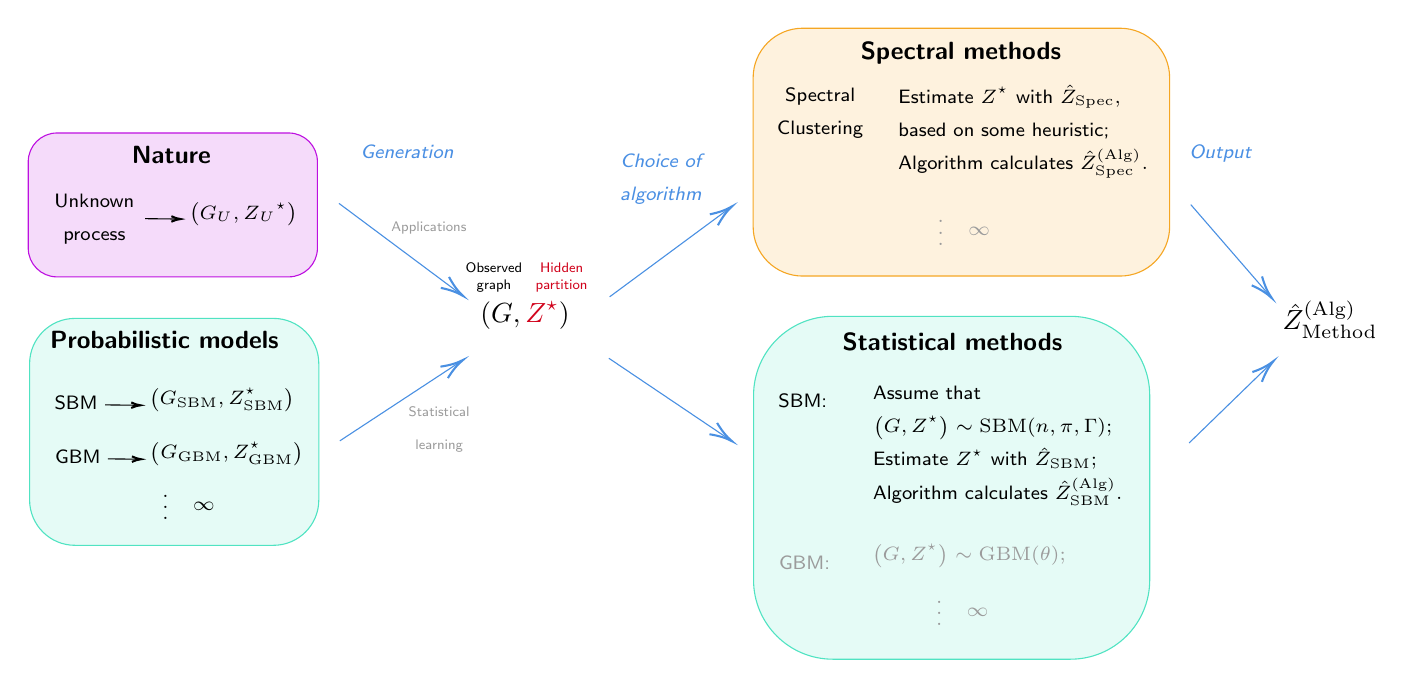
\begin{tikzpicture}[x=0.75pt,y=0.75pt,yscale=-1,xscale=1]
%uncomment if require: \path (0,340); %set diagram left start at 0, and has height of 340


%Rounded Rect [id:dp5598678859389151] 
\draw  [color={rgb, 255:red, 189; green, 16; blue, 224 }  ,draw opacity=1 
][fill={rgb, 255:red, 189; green, 16; blue, 224 }  ,fill opacity=0.15 ] (0.67,66.53) 
.. controls (0.67,58.87) and (6.87,52.67) .. (14.53,52.67) -- (126.13,52.67) .. 
controls (133.79,52.67) and (140,58.87) .. (140,66.53) -- (140,108.13) .. 
controls (140,115.79) and (133.79,122) .. (126.13,122) -- (14.53,122) .. 
controls (6.87,122) and (0.67,115.79) .. (0.67,108.13) -- cycle ;

%Rounded Rect [id:dp2998493990810811] 
\draw  [color={rgb, 255:red, 80; green, 227; blue, 194 }  ,draw opacity=1
][fill={rgb, 255:red, 80; green, 227; blue, 194 }  ,fill opacity=0.15 ] 
(1.33,163.87) .. controls (1.33,151.79) and (11.12,142) .. (23.2,142) -- 
(118.8,142) .. controls (130.88,142) and (140.67,151.79) .. (140.67,163.87) -- 
(140.67,229.47) .. controls (140.67,241.54) and (130.88,251.33) .. 
(118.8,251.33) -- (23.2,251.33) .. controls (11.12,251.33) and (1.33,241.54) .. 
(1.33,229.47) -- cycle ;

%Straight Lines [id:da020709650410012714] 
\draw [color={rgb, 255:red, 74; green, 144; blue, 226 }  ,draw opacity=1]   
(150.4,86.6) -- (208.6,130) ;
\draw [shift={(210.2,131.2)}, rotate = 216.72] [color={rgb, 255:red, 74; green, 144; blue, 226 }  ,draw opacity=1 ][line width=0.75]    (10.93,-3.29) .. controls (6.95,-1.4) and (3.31,-0.3) .. (0,0) .. controls (3.31,0.3) and (6.95,1.4) .. (10.93,3.29)   ;
%Straight Lines [id:da7899960226161649] 
\draw [color={rgb, 255:red, 74; green, 144; blue, 226 }  ,draw opacity=1 ]   (150.8,201) -- (208.53,163.1) ;
\draw [shift={(210.2,162)}, rotate = 146.71] [color={rgb, 255:red, 74; green, 144; blue, 226 }  ,draw opacity=1 ][line width=0.75]    (10.93,-3.29) .. controls (6.95,-1.4) and (3.31,-0.3) .. (0,0) .. controls (3.31,0.3) and (6.95,1.4) .. (10.93,3.29)   ;
%Straight Lines [id:da16550711804548124] 
\draw [color={rgb, 255:red, 74; green, 144; blue, 226 }  ,draw opacity=1 ]   (280.8,131.6) -- (338.19,89.19) ;
\draw [shift={(339.8,88)}, rotate = 143.54] [color={rgb, 255:red, 74; green, 144; blue, 226 }  ,draw opacity=1 ][line width=0.75]    (10.93,-3.29) .. controls (6.95,-1.4) and (3.31,-0.3) .. (0,0) .. controls (3.31,0.3) and (6.95,1.4) .. (10.93,3.29)   ;
%Straight Lines [id:da04365340761949632] 
\draw [color={rgb, 255:red, 74; green, 144; blue, 226 }  ,draw opacity=1 ]   (280.4,161.2) -- (338.14,200.08) ;
\draw [shift={(339.8,201.2)}, rotate = 213.96] [color={rgb, 255:red, 74; green, 144; blue, 226 }  ,draw opacity=1 ][line width=0.75]    (10.93,-3.29) .. controls (6.95,-1.4) and (3.31,-0.3) .. (0,0) .. controls (3.31,0.3) and (6.95,1.4) .. (10.93,3.29)   ;
%Rounded Rect [id:dp6389998939455174]  %% BIG RECTANGLE
\draw  [color={rgb, 255:red, 80; green, 227; blue, 194 }  ,draw opacity=1 
][fill={rgb, 255:red, 80; green, 227; blue, 194 }  ,fill opacity=0.15 ] 
(350.13,179.17) .. controls (350.13,158.09) and (367.22,141) .. (388.31,141) 
-- (502.83,141) .. controls (523.91,141) and (541,158.09) .. (541,179.17) -- 
(541,268.03) .. controls (541,289.11) and (523.91,306.2) .. (502.83,306.2) -- 
(388.31,306.2) .. controls (367.22,306.2) and (350.13,289.11) .. 
(350.13,268.03) -- cycle ;

%Rounded Rect [id:dp6389998939455174]  %% BIG RECTANGLE SAVE
%\draw  [color={rgb, 255:red, 80; green, 227; blue, 194 }  ,draw opacity=1 
%][fill={rgb, 255:red, 80; green, 227; blue, 194 }  ,fill opacity=0.15 ] 
%(350.13,179.17) .. controls (350.13,158.09) and (367.22,141) .. (388.31,141) 
%-- (502.83,141) .. controls (523.91,141) and (541,158.09) .. (541,179.17) -- 
%(541,298.03) .. controls (541,319.11) and (523.91,336.2) .. (502.83,336.2) -- 
%(388.31,336.2) .. controls (367.22,336.2) and (350.13,319.11) .. 
%(350.13,298.03) -- cycle ;

%Rounded Rect [id:dp566655053637461] 
\draw  [color={rgb, 255:red, 245; green, 166; blue, 35 }  ,draw opacity=1 ][fill={rgb, 255:red, 245; green, 166; blue, 35 }  ,fill opacity=0.15 ] (349.93,26.08) .. controls (349.93,12.89) and (360.62,2.2) .. (373.81,2.2) -- (526.72,2.2) .. controls (539.91,2.2) and (550.6,12.89) .. (550.6,26.08) -- (550.6,97.72) .. controls (550.6,110.91) and (539.91,121.6) .. (526.72,121.6) -- (373.81,121.6) .. controls (360.62,121.6) and (349.93,110.91) .. (349.93,97.72) -- cycle ;
%Straight Lines [id:da03352159203926264] 
\draw [color={rgb, 255:red, 74; green, 144; blue, 226 }  ,draw opacity=1 ]   (560.8,87.2) -- (598.49,130.69) ;
\draw [shift={(599.8,132.2)}, rotate = 229.09] [color={rgb, 255:red, 74; green, 144; blue, 226 }  ,draw opacity=1 ][line width=0.75]    (10.93,-3.29) .. controls (6.95,-1.4) and (3.31,-0.3) .. (0,0) .. controls (3.31,0.3) and (6.95,1.4) .. (10.93,3.29)   ;
%Straight Lines [id:da1598730233416068] 
\draw [color={rgb, 255:red, 74; green, 144; blue, 226 }  ,draw opacity=1 ]   (560,202) -- (599.16,163.99) ;
\draw [shift={(600.6,162.6)}, rotate = 135.86] [color={rgb, 255:red, 74; green, 144; blue, 226 }  ,draw opacity=1 ][line width=0.75]    (10.93,-3.29) .. controls (6.95,-1.4) and (3.31,-0.3) .. (0,0) .. controls (3.31,0.3) and (6.95,1.4) .. (10.93,3.29)   ;

% Text Node
\draw (217.27,132.53) node [anchor=north west][inner sep=0.75pt]   [align=left] {$\displaystyle \left( G,\textcolor[rgb]{0.82,0.01,0.11}{Z^{\star }}\right)$};
% Text Node
\draw (208.93,114.2) node [anchor=north west][inner sep=0.75pt]   [align=left] 
{\begin{minipage}[lt]{22.33pt}\setlength\topsep{0pt}
\begin{center}
{\fontfamily{cmss}\selectfont {\tiny 
Observed}}\\[-6pt]{\fontfamily{cmss}\selectfont 
{\tiny graph}}
\end{center}

\end{minipage}};
% Text Node
\draw (242.6,114.2) node [anchor=north west][inner sep=0.75pt]  [color={rgb, 
255:red, 208; green, 2; blue, 27 }  ,opacity=1 ] [align=left] 
{\begin{minipage}[lt]{20.72pt}\setlength\topsep{0pt}
\begin{center}
{\fontfamily{cmss}\selectfont {\tiny 
Hidden}}\\[-6pt]{\fontfamily{cmss}\selectfont 
{\tiny partition}}
\end{center}

\end{minipage}};
% Text Node
\draw (49.33,57.67) node [anchor=north west][inner sep=0.75pt]   [align=left] 
{{\small {\fontfamily{cmss}\selectfont \textbf{Nature}}}};
% Text Node
\draw (11,80.67) node [anchor=north west][inner sep=0.75pt]   [align=left] {\begin{minipage}[lt]{30.44pt}\setlength\topsep{0pt}
\begin{center}
{\scriptsize {\fontfamily{cmss}\selectfont 
Unknown}}\\{\fontfamily{cmss}\selectfont {\scriptsize process}}
\end{center}

\end{minipage}};
% Text Node
\draw (77,85) node [anchor=north west][inner sep=0.75pt]   [align=left] {{\scriptsize $\displaystyle \left( G_{U} ,Z{_{U}}^{\star }\right)$}};
% Text Node
\draw (10,147) node [anchor=north west][inner sep=0.75pt]   [align=left] 
{{\fontfamily{cmss}\selectfont {\small \textbf{Probabilistic models}}}};
% Text Node
\draw (10.67,178) node [anchor=north west][inner sep=0.75pt]   [align=left] {\begin{minipage}[lt]{17.69pt}\setlength\topsep{0pt}
\begin{center}
{\fontfamily{cmss}\selectfont {\scriptsize SBM}}
\end{center}

\end{minipage}};
% Text Node
\draw (57.67,174.33) node [anchor=north west][inner sep=0.75pt]   [align=left] 
{{\scriptsize $\displaystyle \left( G_{\text{SBM}} ,Z_{\text{SBM}}^{\star }\right)$}};
% Text Node
\draw (11,204) node [anchor=north west][inner sep=0.75pt]   [align=left] {\begin{minipage}[lt]{18.48pt}\setlength\topsep{0pt}
\begin{center}
{\fontfamily{cmss}\selectfont {\scriptsize GBM}}
\end{center}

\end{minipage}};
% Text Node
\draw (58,200.33) node [anchor=north west][inner sep=0.75pt]   [align=left] 
{{\scriptsize $\displaystyle \left( G_{\text{GBM}} ,Z_{\text{GBM}}^{\star 
}\right)$}};
% Text Node
\draw (64,218) node [anchor=north west][inner sep=0.75pt]   [align=left] 
{{\scriptsize $\displaystyle \vdots $}};
% Text Node
\draw (78.67,229.33) node [anchor=north west][inner sep=0.75pt]   [align=left] 
{{\scriptsize $\displaystyle \infty $}};
% Text Node
\draw (159.6,57.4) node [anchor=north west][inner sep=0.75pt]   [align=left] 
{\textit{{\scriptsize {\fontfamily{cmss}\selectfont 
\textcolor[rgb]{0.29,0.56,0.89}{Generation}}}}};
% Text Node
\draw (174.4,94.4) node [anchor=north west][inner sep=0.75pt]  [color={rgb, 
255:red, 155; green, 155; blue, 155 }  ,opacity=1 ] [align=left] 
{{\fontfamily{cmss}\selectfont {\tiny Applications}}};
% Text Node
\draw (181.5,183.5) node [anchor=north west][inner sep=0.75pt]  [color={rgb, 255:red, 155; green, 155; blue, 155 }  ,opacity=1 ] [align=left] {\begin{minipage}[lt]{23.85pt}\setlength\topsep{0pt}
\begin{center}
{\fontfamily{cmss}\selectfont {\tiny Statistical}}\\{\fontfamily{cmss}\selectfont 
{\tiny learning}}
\end{center}

\end{minipage}};
% Text Node
\draw (283.6,61.4) node [anchor=north west][inner sep=0.75pt]   [align=left] {\begin{minipage}[lt]{30.87pt}\setlength\topsep{0pt}
\begin{center}
\textit{{\scriptsize {\fontfamily{cmss}\selectfont 
\textcolor[rgb]{0.29,0.56,0.89}{Choice of}}}}\\\textit{{\scriptsize 
{\fontfamily{cmss}\selectfont \textcolor[rgb]{0.29,0.56,0.89}{algorithm}}}}
\end{center}

\end{minipage}};
% Text Node
\draw (391.8,148) node [anchor=north west][inner sep=0.75pt]   [align=left] 
{{\fontfamily{cmss}\selectfont {\small \textbf{Statistical methods}}}};
% Text Node
\draw (359.47,177) node [anchor=north west][inner sep=0.75pt]   [align=left] {\begin{minipage}[lt]{19.67pt}\setlength\topsep{0pt}
\begin{center}
{\fontfamily{cmss}\selectfont {\scriptsize SBM:}}
\end{center}

\end{minipage}};
% Text Node
\draw (406.47,173.33) node [anchor=north west][inner sep=0.75pt]   
[align=left] {{\scriptsize {\fontfamily{cmss}\selectfont Assume 
that}}\\{\scriptsize 
$\displaystyle \left( G ,Z^{\star }\right) \sim \text{SBM}( n,\pi ,\Gamma ) 
;$}\\{\scriptsize {\fontfamily{cmss}\selectfont Estimate }$\displaystyle Z^{\star 
}$ 
{\fontfamily{cmss}\selectfont with }$\displaystyle 
\hat{Z}_{\text{SBM}}$;}\\{\scriptsize {\fontfamily{cmss}\selectfont Algorithm 
calculates }$\displaystyle \hat{Z}_{\text{SBM}}^{\text{(Alg)}}$.}};
% Text Node
\draw (359.8,255) node [anchor=north west][inner sep=0.75pt]  [color={rgb, 
255:red, 155; green, 155; blue, 155 }  ,opacity=1 ] [align=left] 
{\begin{minipage}[lt]{20.47pt}\setlength\topsep{0pt}
\begin{center}
{\fontfamily{cmss}\selectfont {\scriptsize GBM:}}
\end{center}

\end{minipage}};
% Text Node
\draw (436.8,269) node [anchor=north west][inner sep=0.75pt]  [color={rgb, 
255:red, 155; green, 155; blue, 155 }  ,opacity=1 ] [align=left] {{\scriptsize 
$\displaystyle \vdots $}};
% Text Node
\draw (451.47,280.33) node [anchor=north west][inner sep=0.75pt]  
[color={rgb, 255:red, 155; green, 155; blue, 155 }  ,opacity=1 ] [align=left] 
{{\scriptsize $\displaystyle \infty $}};
% Text Node
\draw (406.07,249.53) node [anchor=north west][inner sep=0.75pt]  
[color={rgb, 255:red, 155; green, 155; blue, 155 }  ,opacity=1 ] [align=left] 
{{\scriptsize $\displaystyle \left( G , Z^{\star }\right) \sim \text{GBM}( \theta ) 
;$}};
% Text Node
\draw (400.6,7.67) node [anchor=north west][inner sep=0.75pt]   [align=left] 
{{\fontfamily{cmss}\selectfont {\small \textbf{Spectral methods}}}};
% Text Node
\draw (359.27,29.67) node [anchor=north west][inner sep=0.75pt]   [align=left] {\begin{minipage}[lt]{32.58pt}\setlength\topsep{0pt}
\begin{center}
{\fontfamily{cmss}\selectfont {\scriptsize 
Spectral}}\\{\fontfamily{cmss}\selectfont {\scriptsize Clustering}}
\end{center}

\end{minipage}};
% Text Node
\draw (437.6,85.67) node [anchor=north west][inner sep=0.75pt]  [color={rgb, 
255:red, 155; green, 155; blue, 155 }  ,opacity=1 ] [align=left] {{\scriptsize 
$\displaystyle \vdots $}};
% Text Node
\draw (452.27,97) node [anchor=north west][inner sep=0.75pt]  [color={rgb, 
255:red, 155; green, 155; blue, 155 }  ,opacity=1 ] [align=left] {{\scriptsize 
$\displaystyle \infty $}};
% Text Node
\draw (418.67,28.13) node [anchor=north west][inner sep=0.75pt]   [align=left] 
{{\scriptsize {\fontfamily{cmss}\selectfont Estimate }$\displaystyle Z^{\star }$ 
{\fontfamily{cmss}\selectfont with }$\displaystyle 
\hat{Z}_{\text{Spec}}$,}\\{\scriptsize {\fontfamily{cmss}\selectfont based on 
some 
heuristic;}}\\{\scriptsize {\fontfamily{cmss}\selectfont Algorithm calculates 
}$\displaystyle \hat{Z}_{\text{Spec}}^{\text{(Alg)}} .$}};
% Text Node
\draw (603.8,132.4) node [anchor=north west][inner sep=0.75pt]   [align=left] 
{$\displaystyle \hat{Z}_{\text{Method}}^{\text{(Alg)}}$};
% Text Node
\draw (558.8,57.4) node [anchor=north west][inner sep=0.75pt]   [align=left] 
{\textit{{\scriptsize {\fontfamily{cmss}\selectfont 
\textcolor[rgb]{0.29,0.56,0.89}{Output}}}}};
% Connection
\draw    (57,93.95) -- (72,94.12) ;
\draw [shift={(74,94.14)}, rotate = 180.65] [color={rgb, 255:red, 0; green, 0; blue, 0 }  ][line width=0.75]    (4.37,-1.32) .. controls (2.78,-0.56) and (1.32,-0.12) .. (0,0) .. controls (1.32,0.12) and (2.78,0.56) .. (4.37,1.32)   ;
% Connection
\draw    (37.67,183.67) -- (52.67,183.84) ;
\draw [shift={(54.67,183.87)}, rotate = 180.65] [color={rgb, 255:red, 0; green, 0; blue, 0 }  ][line width=0.75]    (4.37,-1.32) .. controls (2.78,-0.56) and (1.32,-0.12) .. (0,0) .. controls (1.32,0.12) and (2.78,0.56) .. (4.37,1.32)   ;
% Connection
\draw    (39,209.68) -- (53,209.83) ;
\draw [shift={(55,209.86)}, rotate = 180.65] [color={rgb, 255:red, 0; green, 0; blue, 0 }  ][line width=0.75]    (4.37,-1.32) .. controls (2.78,-0.56) and (1.32,-0.12) .. (0,0) .. controls (1.32,0.12) and (2.78,0.56) .. (4.37,1.32)   ;

\end{tikzpicture}
\end{document}